\chapter{Въведение в алгоритмите и асимптотичния анализ}

\section{Що е то алгоритъм?}

Алгоритмите се срещат навсякъде около нас:
\begin{itemize}
  \item рецептите са алгоритми за готвене
  \item сутрешното приготвяне
  \item придвижването от точка A до точка B
  \item търсенето на книга в библиотеката
\end{itemize}

Въпреки това е трудно да се даде формална дефиниция на това какво точно е алгоритъм.
На ниво интуиция, човек може да си мисли, че това просто е някакъв последователен списък от стъпки/инструкции, които човек/машина трябва да изпълни.
Други начини човек да си мисли за алгоритмите, са:
\begin{itemize}
  \item програми -- обикновено така се реализират алгоритми
  \item машини на Тюринг, крайни (стекови) автомати или формални граматики
  \item частично рекурсивни функции
\end{itemize}

Един програмист в ежедневието си постоянно пише алгоритми за да решава различни задачи/проблеми.
Една задача може да се решава по много начини, някои по-добри от други.
Добрият програмист, освен че ще намери решение на проблема, той ще намери най-доброто решение (или поне достатъчно добро за неговите цели).

\section{Какво означава добро решение?}

Хубаво е човек да се води по следните (неизчерпателни) критерии:
\begin{itemize}
  \item решението трябва да е коректно -- ако алгоритъмът работи само през 50\% от времето, най-вероятно можем да се справим по-добре
  \item решението трябва да е бързо -- ако алгоритъмът ще завърши работа след като всички звезди са измрели, то той практически не ни върши работа
  \item решението трябва да заема малко памет -- ако алгоритъмът по време на своята работа се нуждае от повече памет, колкото компютърът може да предостави, за нас този алгоритъм е безполезен
  \item решението трябва да е просто -- това е може би най-маловажният критерии от тези, но въпреки това е хубаво когато човек може, да пише чист и разбираем код, който лесно се разширява
\end{itemize}

За да можем да сравняваме алгоритми в зависимост от това колко големи ресурси (време и памет) използват, трябва първо да можем да ``измерваме'' тези ресурси.

\section{Как мерим времето и паметта?}

Когато пишем алгоритми, имаме няколко базови инструкции (за които предварително сме се уговорили), които ще наричаме \textbf{атомарни инструкции}.
Тяхното извикване ще отнеме една единица време.
\textbf{Време за изпълнение} ще наричаме броят на извикванията на атомарните инструкции по време на изпълнение на програмата.
Също така числата и символите ще бъдат нашите \textbf{атомарни типове данни}, и ще заемат една единица памет.
\textbf{Паметта}, която една програма заема, ще наричаме максималния брой на единици от атомарни типове данни по време на изпълнение, без да броим входните данни.
Обикновено времето и паметта зависят от размера на подадените входни данни.
Това означава, че можем да си мислим за времето и паметта като функции на размера на входа.
Подходът, който ще изберем, е да сравняваме функциите за време/памет на различните алгоритми асимптотично.
Интересуваме се не толкова от конкретните стойности, а от поведението им, когато размерът на входа клони към безкрайност.

\section{Основни дефиниции}
\footnotetext[1]{точност до константен множител и константно събираемо}
Множеството от функции, които ще анализираме, е
\[
  \calF = \{ f \mid f : \R^{\geq 0} \rightarrow \R \: \& \: (\exists n_0 > 0) (\forall n \geq n_0) (f(n) > 0) \}.
\]


\begin{definition}
  За всяка функция $f \in \calF$ дефинираме:
  \begin{align*}
    \Theta(f) = \{ g \in \calF \: \mid & (\exists c_1 > 0)(\exists c_2 > 0)                                                        \\
                                       & (\exists n_0 \in \N)(\forall n \geq n_0)(c_1 \cdot f(n) \leq g(n) \leq c_2 \cdot f(n))\}.
  \end{align*}

\end{definition}
Може да тълкуваме $\Theta(f)$ като:
\begin{center}
  \textit{``множеството от функциите, които растат\footnotemark[1] със скоростта на $f$''.}
\end{center}


Нека вземем за пример $f(n) = 3n + 1$ и $g(n) = n + 200$:

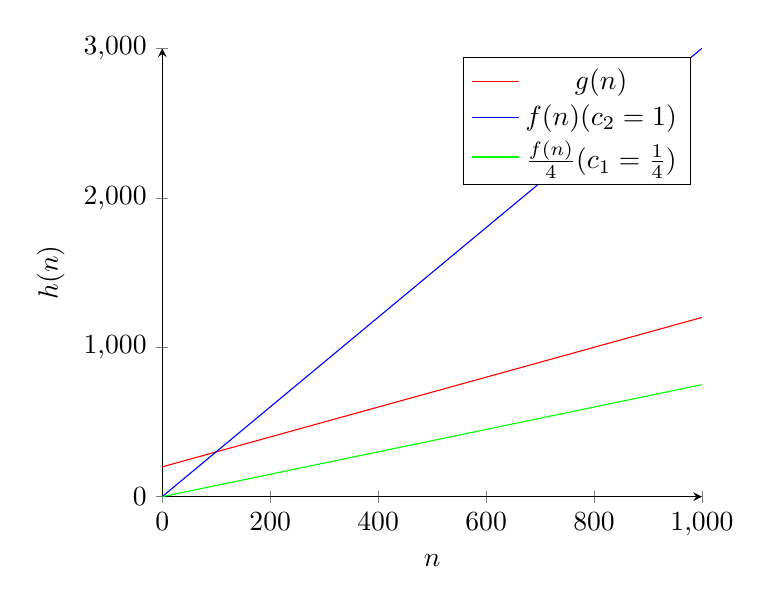
\begin{tikzpicture}
  \begin{axis}[axis lines = left, xlabel = \(n\), ylabel = {\(h(n)\)}]
    \addplot[domain = 0:1000, color=red]{x+200};
    \addlegendentry{$g(n)$};
    \addplot[domain = 0:1000, color=blue]{(3*x)+1};
    \addlegendentry{$f(n) (c_2 = 1)$};
    \addplot[domain = 0:1000, color=green]{((3*x)+1)/4};
    \addlegendentry{$\frac{f(n)}{4} (c_1 = \frac{1}{4})$};
  \end{axis}
\end{tikzpicture}

На картинката се вижда как от един момент нататък, функцията $f$ остава ``заключена`` между $c_1 \cdot g$ и $c_2 \cdot g$.
Точно заради това $g \in \Theta(f)$.
\begin{remark}
  Вместо да пишем $g \in \Theta(f)$, ще пишем $g = \Theta(f)$ или $g \asymp f$.
\end{remark}

\newpage

\begin{definition}
  За всяка функция $f \in \calF$ дефинираме:
  \begin{align*}
    O(f) = \{ g \in \calF \: \mid (\exists c > 0)(\exists n_0 \in \N)(\forall n \geq n_0)(g(n) \leq c \cdot f(n))\}.
  \end{align*}
\end{definition}
Може да тълкуваме $O(f)$ като:
\begin{center}
  \textit{``множеството от функциите, които не растат\footnotemark[1] по-бързо от $f$''.}
\end{center}


Тук заслабваме условията от $\Theta(f)$ като искаме само горната граница.

За пример човек може да вземе $f(n) = n^2$ и $g(n) = n$:

\begin{tikzpicture}
  \begin{axis}[axis lines = left, xlabel = \(n\), ylabel = {\(h(n)\)}]
    \addplot[domain = 0:10, color=red]{x*x};
    \addlegendentry{$f(n)$};
    \addplot[domain = 0:10, color=blue]{x};
    \addlegendentry{$g(n)$};
  \end{axis}
\end{tikzpicture}

\begin{remark}
  Вместо да пишем $g \in O(f)$, ще пишем $g = O(f)$ или $g \preceq f$.
\end{remark}

\begin{definition}
  За всяка функция $f \in \calF$ дефинираме:
  \begin{align*}
    o(f) = \{ g \in \calF \: \mid (\forall c > 0)(\exists n_0 \in \N)(\forall n \geq n_0)(g(n) < c \cdot f(n))\}.
  \end{align*}
\end{definition}
Може да тълкуваме $o(f)$ като:
\begin{center}
  \textit{``множеството от функциите, които растат\footnotemark[1] по-бавно от $f$''.}
\end{center}
Разликата между $O(f)$ и $o(f)$ е строгото неравенство и универсалният квантор в началото.
Лесно се вижда, че $o(f) \subseteq O(f)$.
Тук изключваме функциите от същия порядък.
\begin{remark}
  Вместо да пишем $g \in o(f)$, ще пишем $g = o(f)$ или $g \prec f$.
\end{remark}

\begin{definition}
  За всяка функция $f \in \calF$ дефинираме:
  \begin{align*}
    \Omega(f) = \{ g \in \calF \: \mid (\exists c > 0)(\exists n_0 \in \N)(\forall n \geq n_0)(c \cdot f(n) \leq g(n))\}.
  \end{align*}
\end{definition}
Може да тълкуваме $\Omega(f)$ като:
\begin{center}
  \textit{``множеството от функциите, които не растат\footnotemark[1] по-бавно от $f$''.}
\end{center}
Това е дуалното множество на $O(f)$.
\begin{remark}
  Вместо да пишем $g \in \Omega(f)$, ще пишем $g = \Omega(f)$ или $g \succeq f$.
\end{remark}

\begin{definition}
  За всяка функция $f \in \calF$ дефинираме:
  \begin{align*}
    \omega(f) = \{ g \in \calF \: \mid (\forall c > 0)(\exists n_0 \in \N)(\forall n \geq n_0)(c \cdot f(n) < g(n))\}.
  \end{align*}
\end{definition}
Може да тълкуваме $\omega(f)$ като:
\begin{center}
  \textit{``множеството от функциите, които растат\footnotemark[1] по-бързо от $f$''.}
\end{center}
Това е дуалното множество на $o(f)$.
\begin{remark}
  Вместо да пишем $g \in \omega(f)$, ще пишем $g = \omega(f)$ или $g \succ f$.
\end{remark}

\begin{warning}
  Не всички функции от $\calF$ са сравними по релациите $\prec, \preceq$ или $\asymp$.

  За пример човек може да вземе функциите $f(n) = n$ и $g(n) = n^{1 + \sin(n)}$.
  Лесно се вижда, че функцията $g(n)$ ``плава'' между $n^0 = 1$ и $n^2$ т.е. няма нито как да расте по-бързо, нито как да расте по-бавно.
\end{warning}

Въпреки това, тези релации са сравнително хубави.
\begin{claim}
  Следните свойства са в сила:
  \begin{itemize}
    \item $\asymp$ е релация на еквивалентност;
    \item $\prec$ и $\succ$ са транзитивни и антирефлексивни;
    \item $\preceq$ и $\succeq$ са транзитивни и рефлексивни.
  \end{itemize}
\end{claim}

Доказателството на това твърдение оставяме за упражнение на читателя.
То е една елементарна разходка из дефинициите.

\newpage

\section{Полезни свойства}

Тук ще изброим няколко свойства, които много често се ползват в задачите:
\begin{itemize}
  \item Нека $f, g \in \calF$ и $\lim\limits_{n \rightarrow \infty} \frac{f(n)}{g(n)} = l$ (тук искаме границата да съществува).
        Тогава: \\
        --- ако $l = 0$, то $f \prec g$ \\
        --- ако $l = \infty$, то $f \succ g$ \\
        --- в останалите случаи $f \asymp g$
  \item $f + g \asymp \max\{f, g\}$ за всяко $f, g \in \calF$
  \item $c \cdot f \asymp f$ за всяко $f \in F$ и $c > 0$
  \item $f \asymp g \iff f^c \asymp g^c$ за всяко $f, g \in F$ и $c > 0$
  \item $O(f) \cap \Omega(f) = \Theta(f)$ за всяко $f \in \calF$
  \item $o(f) \cap \omega(f) = O(f) \cap \omega(f) = o(f) \cap \Omega(f) = \varnothing$ за всяко $f \in \calF$
  \item $f \prec g \iff g \succ f$ и $f \preceq g \iff g \succeq f$ за всяко $f, g \in \calF$
  \item ако $f \prec g$, то $c^f \prec c^g$ за всяко $f, g \in \calF$ и $c > 1$
  \item ако $\log_c(f) \prec \log_c(g)$, то $f \prec g$ за всяко $f, g \in \calF$ и $c > 1$
  \item ако $c^f \asymp c^g$, то $f \asymp g$ за всяко $f, g \in \calF$ и $c > 1$
  \item ако $f \asymp g$, то $\log_c(f) \asymp \log_c(g)$ за всяко $f, g \in \calF$ и $c > 1$
  \item тъй като $\log_a(n) = \frac{\log_b(n)}{\log_b(a)}$, то $\log_a(n) \asymp \log_b(n)$ -- вече ще пишем само $\log(n)$ като ще имаме предвид $\log_2(n)$
  \item $n! \asymp \sqrt{n} \frac{n^n}{e^n}$ - апроксимация на Стирлинг
  \item $\log(n!) \asymp n \log(n)$
  \item $\log(n) \prec n^k \prec 2^n \prec n! \prec n^n \prec 2^{n^2}$ за всяко $k \geq 1$
\end{itemize}

\section{Задачи}

\begin{problem}
Да се сравнят асимптотично следните двойки функции:
\begin{enumerate}
  \item $f(n) = \log(\log(n))$ и $g(n) = \log(n)$
  \item $f(n) = 5n^3$ и $g(n) = n \sqrt{n^9 + n^5}$
  \item $f(n) = n 5^n$ и $g(n) = n^ 2 3^n$
  \item $f(n) = n^n$ и $g(n) = 3^{n^2}$
  \item $f(n) = 3^{n^2}$ и $g(n) = 2^{n^3}$
\end{enumerate}
\end{problem}

\begin{problem}
Да се докаже, че $\sum\limits_{i = 0}^n i^k \asymp n^{k+1}$
\end{problem}

\begin{problem}
Да се подредят по асимптотично нарастване следните функции:
\begin{align*}
  f_1(n) & = n^2                                       & f_2(n)    & = \sqrt{n}       & f_3(n)    & = \log^2(n)        & f_4(n)    & = \sqrt{\log(n)!}                         \\
  f_5(n) & = \sum\limits_{k = 2}^{\log(n)} \frac{1}{k} & f_6(n)    & = \log(\log(n))  & f_7(n)    & = 2^{2^{\sqrt{n}}} & f_8(n)    & = \binom{\binom{n}{3}}{2}                 \\
  f_9(n) & =2^{n^2}                                    & f_{10}(n) & = 3^{n \sqrt{n}} & f_{11}(n) & =2^{\binom{n}{2}}  & f_{12}(n) & = \sum\limits_{k = 1}^{n^2} \frac{1}{2^k}
\end{align*}
\end{problem}